\documentclass{article}
\usepackage[utf8]{inputenc}
\usepackage{fancyhdr}
\usepackage{graphicx}
\usepackage{pdflscape}
\usepackage[margin=0.75in]{geometry}
 
\pagestyle{fancy}
\fancyhf{}
\rhead{Rachel LeCover}
\lhead{Biokinetics Problem Set 2}
\rfoot{Page \thepage}
 
\begin{document}
 
\section*{Problem 1}
I confirmed that my network was balanced through the use of \texttt{checkAllBalances()}, a function which goes through all reactions in the network and confirms that an equal number of atoms of each species are found as reactants and products. Reactions where a species disappears (exchange fluxes) are not balanced, and neither is the biomass production reaction, as biomass is a fictitious species, used to quantify cell growth. Through the use of dynamic flux analysis and the bounds given on oxygen update, glucose uptake, and growth rate, I was able to predict with a high degree of accuracy the rate at which E. coli would uptake glucose, as shown in Figure \ref{fig:aerobic}. By setting the maximum oxygen uptake rate to zero, I was able to predict the anaerobic fluxes, as shown in Figure \ref{fig:anaerobic}. I used an initial biomass concentration of .001 g/L, since this gave a good fit to the glucose uptake and biomass curve, since no initial value was given by Palsson. Initial concentrations of all species other than glucose and acetate were assumed to be zero, and initial concentrations of glucose and acetate were set based on the data in figure 7 of \cite{varma1994stoichiometric}.

To perform dynamic flux balance analysis (dFBA), I solved
\begin{equation}
\frac{dX}{dt} = Sv
\end{equation}
where $X$ gives the species concentrations as a function of time, $S$ is the stoichiometric matrix, and $v$ represents the fluxes through the network, as determined by FBA. This equation neglects the growth and dilution terms in a complete mass balance, as they are small. I solved the differential equation using Euler's method with a time step of .1 hours.  For the purposes of FBA, I formulated my objective as maximizing the flux through the biomass producing reaction.
\begin{figure}[!h]
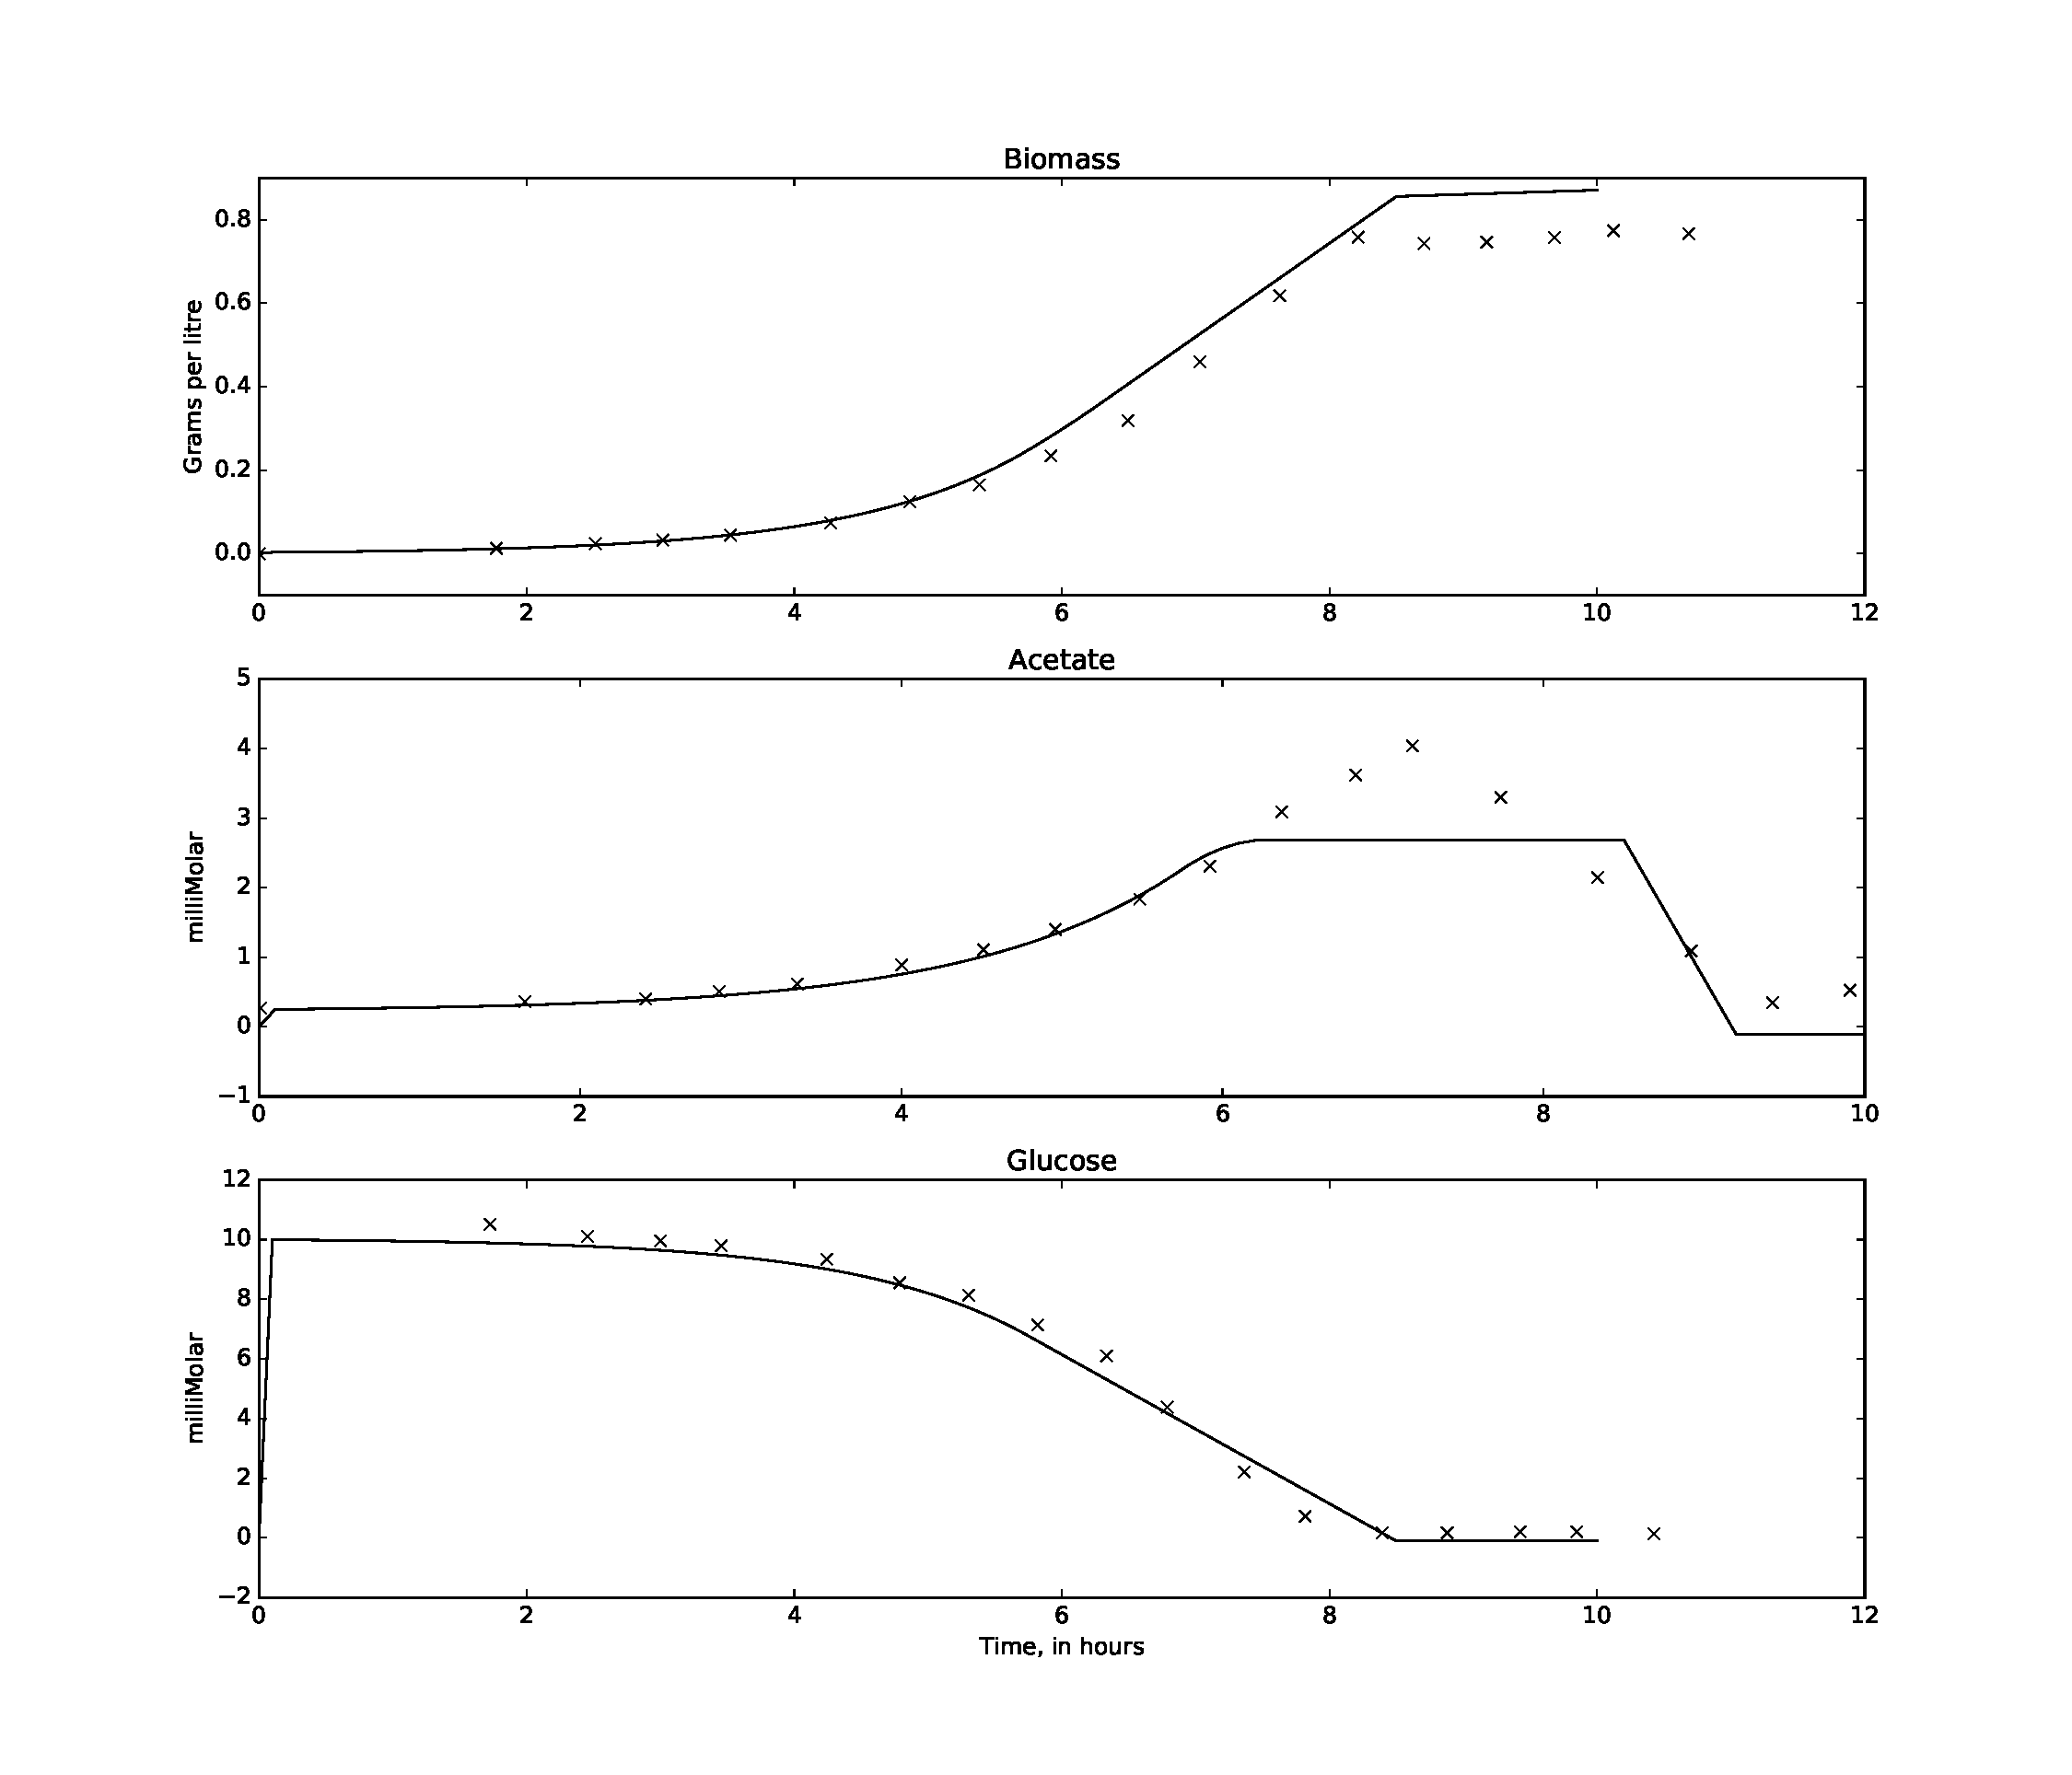
\includegraphics[width=18cm]{../MikesNewNetwork/figures/AttemptToRecreateFig7}
\caption{Concentrations of selected metabolites as a function of time as calculated by dFBA, grown in a batch culture in the pretense of oxygen. Lines show predicted data, xs show experimental data extracted from \cite{varma1994stoichiometric}.}
\label{fig:aerobic}
\end{figure}

\begin{figure}[!h]
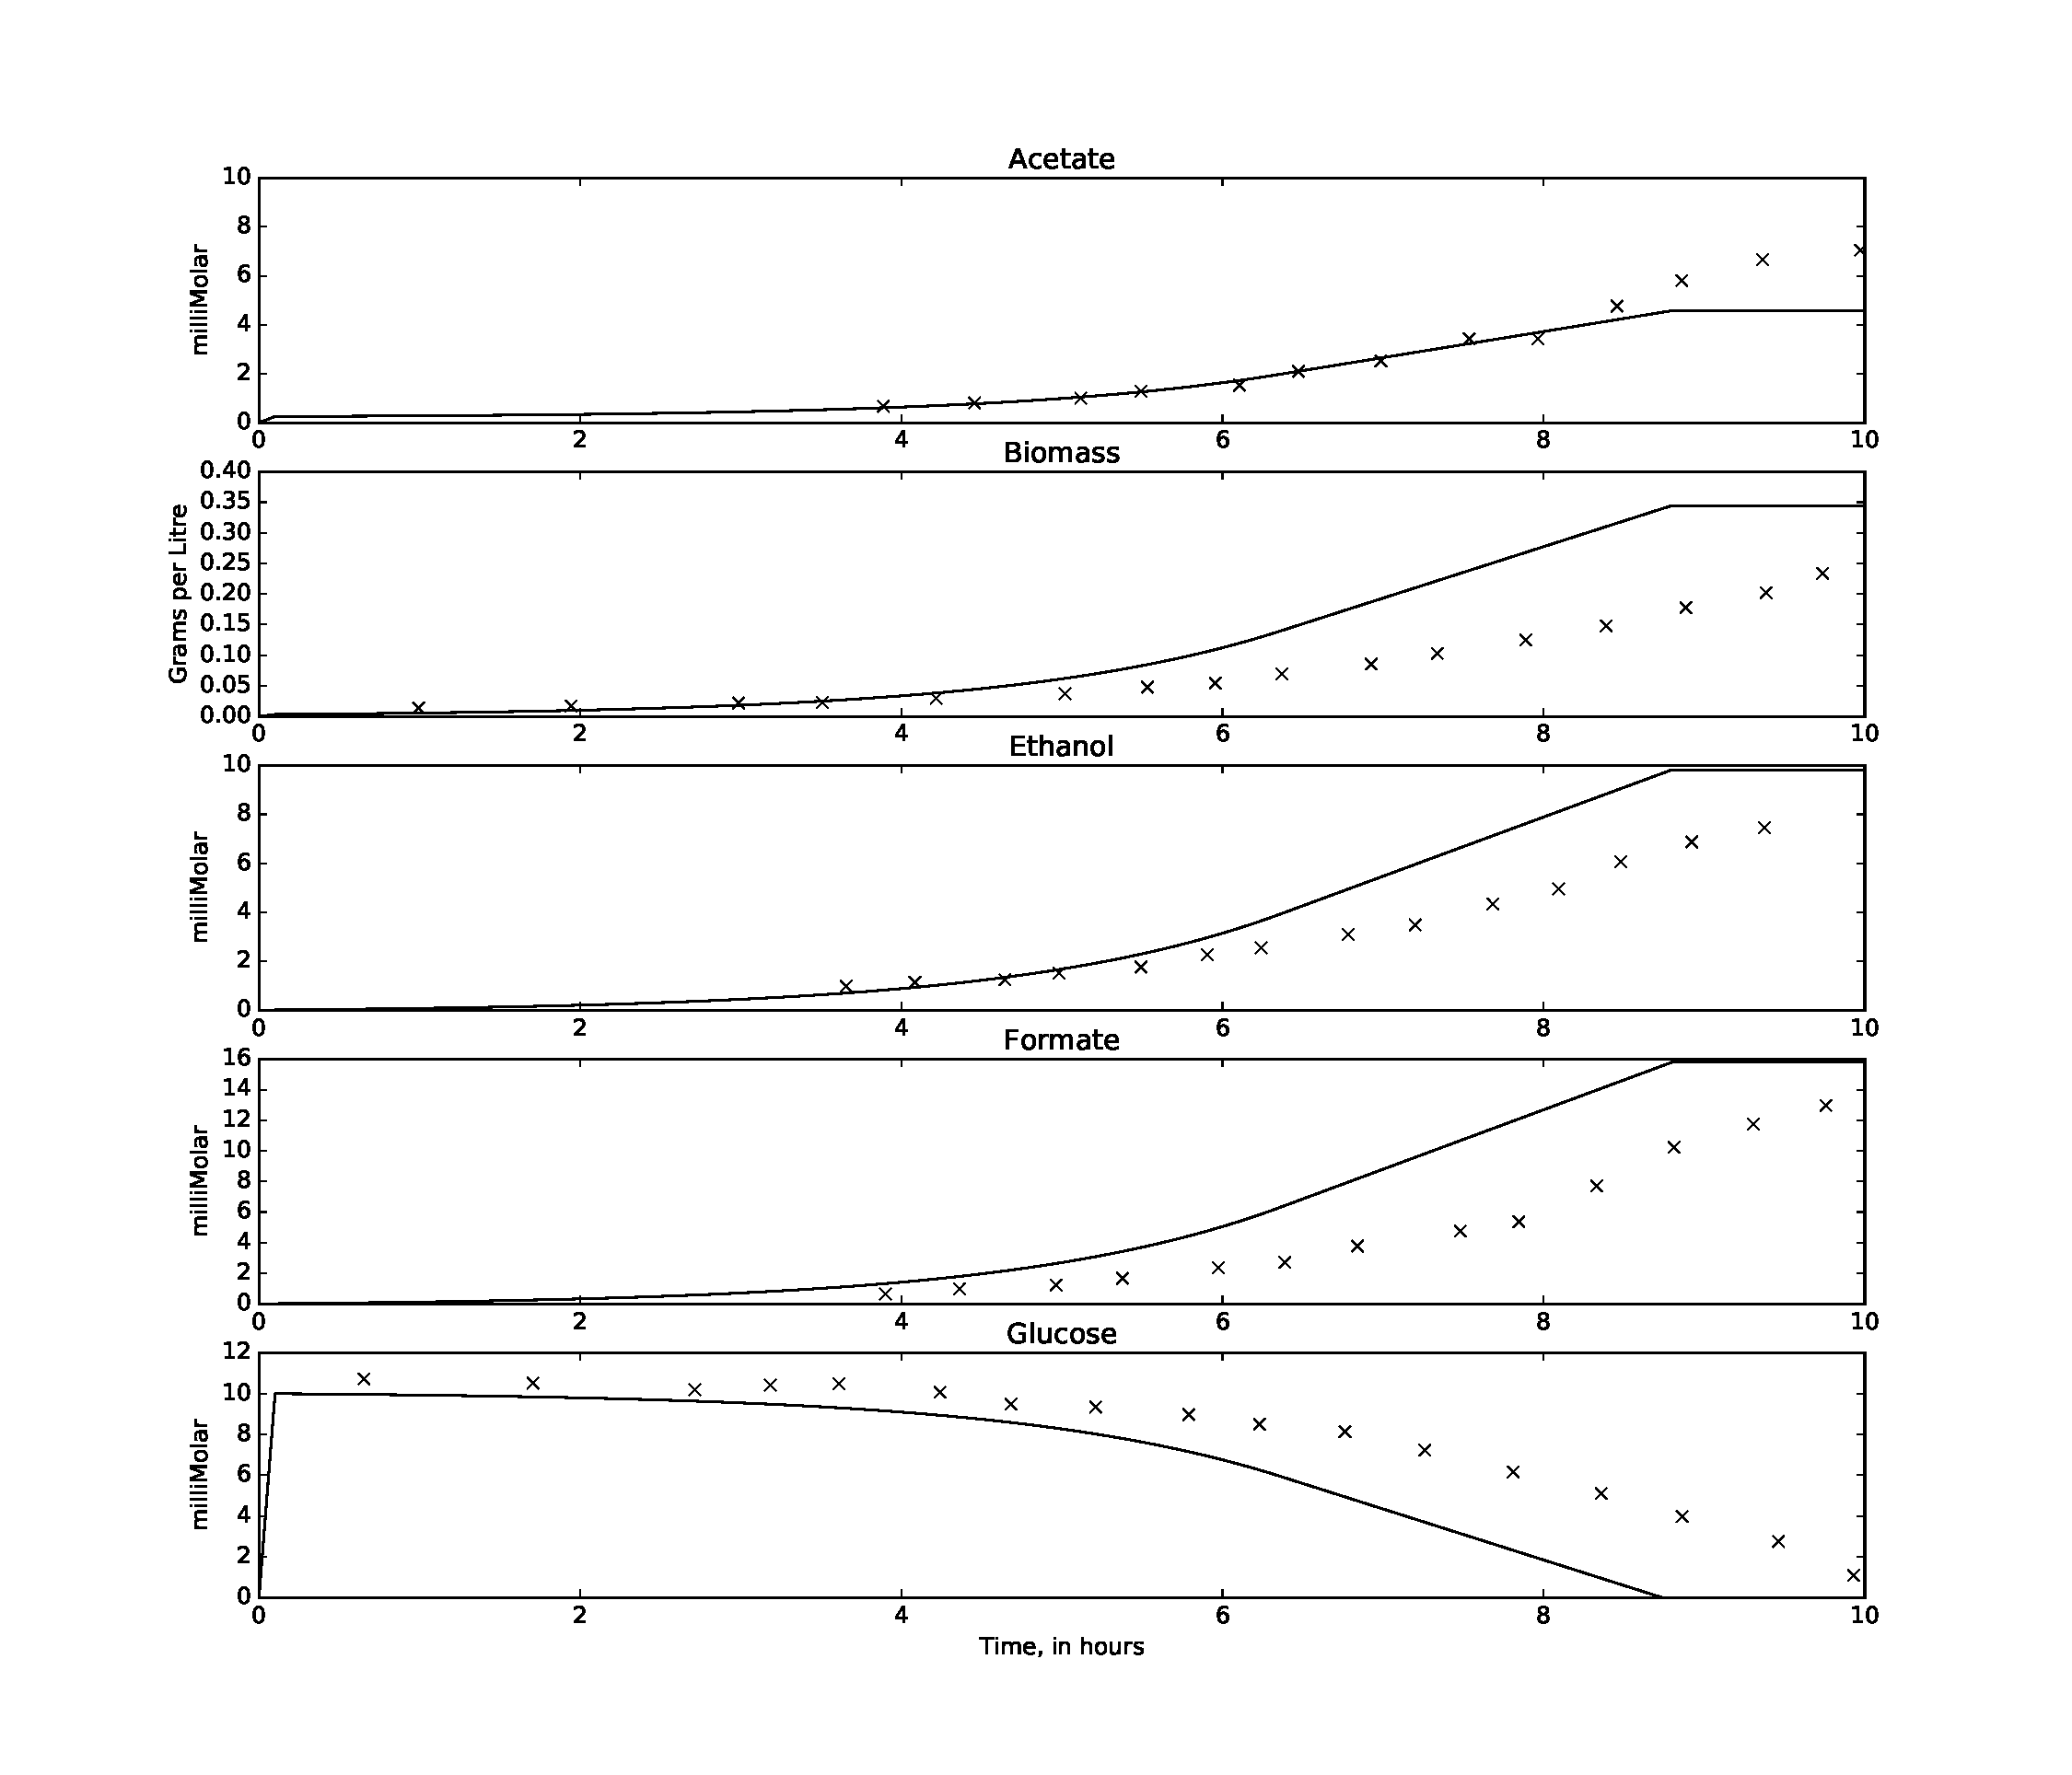
\includegraphics[width=18cm]{../MikesNewNetwork/figures/AttemptToRecreateFig11}
\caption{Concentrations of selected metabolites as a function of time as calculated by dFBA, grown in a batch culture in the absense of oxygen. Lines show predicted data, xs show experimental data extracted from \cite{varma1994stoichiometric}. }
\label{fig:anaerobic}
\end{figure}
There are two ways in which E. coli can generate ATP-through substrate level phosphorylation and oxidative phosphorylation. Substrate level phosphorylation generates ATP by reactions between organic molecules, whereas oxidative phosphorlation uses ATP synthase with a proton gradient to produce ATP \cite{conway2015metabolism}. When E. coli uptake glucose, they invest two ATP convert it to pyruvate, though either gycolysis, pentose phosphate, or Entner Doudoroff pathways. Going through glycolysis increases the amount of ATP available, as it produces 2 ATP for each glucose molecule processed. If oxygen is not present, this pyruvate is used for fermentation, which uses substrate level phosphorlation to produce ATP. While fermentation is faster than oxidative phosphorlation, it is not as energetically efficient \cite{conway2015metabolism}. When oxygen is available, the pyruvate generated through glycolysis can continue through the citric acid cycle, which produces NADH that carries electrons the electron transport chain (which requires an electron acceptor, like oxygen to run), which produces the proton gradient necessary to run ATP synthase \cite{biobook}. 

If we examine the flux profiles in the aerobic and aerobic environments, without applying the bounds given by Palsson's experimental data, we observe that glucose uptake rates are the same, but the flux through biomass production is much larger in the aerobic case, suggesting that energetic species are available for non-essential reactions, like growth. \texttt{R\_atp}, which is represents the creation of ATP by ATP  has no flux through it in the anaerobic case, as expected, and a fairly large flux through it in the pretense of oxygen. Instead, there is a higher flux through reactions that produce ATP through substrate level phosphorolation such as \texttt{R\_pgk} and \texttt{R\_pyk}. Furthermore, in the anaerobic case, ethanol and formate are exported from the cell, which is not observed in the aerobic case. The complete flux profiles for both cases are given in the supplemental material.   
   
\newpage
\bibliography{PS2} 
\bibliographystyle{ieeetr}
\newpage
\begin{landscape}
\section*{Supplemental Material}
\subsection*{Steady State Fluxes in Aerobic Environment}

\begin{verbatim}
1,R_glk_hex::M_pep_c+M_glc_D_e --> M_pyr_c+M_g6p_c,2.5
3,R_pgi::M_g6p_c --> M_f6p_c,1.1041123916076936
5,R_pfk::M_atp_c+M_f6p_c --> M_adp_c+M_fdp_c,1.8270632175924555
7,R_fbaA::M_fdp_c --> M_dhap_c+M_g3p_c,1.8270632175924555
9,R_tpiA::M_dhap_c --> M_g3p_c,1.8270632175924555
11,R_gapA::M_g3p_c+M_nad_c+M_pi_c --> M_13dpg_c+M_h_c+M_nadh_c,3.9541747758961754
13,R_pgk::M_13dpg_c+M_adp_c --> M_3pg_c+M_atp_c,3.9541747758961754
15,R_gpm::M_3pg_c --> M_2pg_c,3.6188531187805015
17,R_eno::M_2pg_c --> M_h2o_c+M_pep_c,3.6188531187805015
19,R_pyk::M_adp_c+M_pep_c --> M_atp_c+M_pyr_c,0.3601878695562891
21,R_ppc::M_co2_c+M_h2o_c+M_pep_c --> M_oaa_c+M_pi_c,0.6423113239509861
22,R_pdh::M_coa_c+M_nad_c+M_pyr_c --> M_accoa_c+M_co2_c+M_nadh_c+M_h_c,2.2252285177666624
24,R_zwf::M_g6p_c+M_nadp_c --> M_6pgl_c+M_h_c+M_nadph_c,1.3499377823838083
26,R_pgl::M_6pgl_c+M_h2o_c --> M_6pgc_c,1.3499377823838083
27,R_gnd::M_6pgc_c+M_nadp_c --> M_co2_c+M_nadph_c+M_ru5p_D_c+M_h_c,1.3499377823838081
28,R_rpe::M_ru5p_D_c --> M_xu5p_D_c,0.7388427414189204
31,R_rpi_reverse::M_ru5p_D_c --> M_r5p_c,0.6110950409648879
32,R_talAB::M_g3p_c+M_s7p_c --> M_e4p_c+M_f6p_c,0.409879632146211
34,R_tkt1::M_r5p_c+M_xu5p_D_c --> M_g3p_c+M_s7p_c,0.409879632146211
36,R_tkt2::M_e4p_c+M_xu5p_D_c --> M_f6p_c+M_g3p_c,0.32896310927270944
40,R_gltA::M_accoa_c+M_h2o_c+M_oaa_c --> M_cit_c+M_coa_c,1.3851760401342272
41,R_acn::M_cit_c --> M_icit_c,1.3851760401342272
43,R_icd::M_icit_c+M_nadp_c --> M_akg_c+M_co2_c+M_nadph_c+M_h_c,1.3851760401342272
45,R_sucAB::M_akg_c+M_coa_c+M_nad_c --> M_co2_c+M_nadh_c+M_succoa_c+M_h_c,1.1433454680338926
46,R_sucCD::M_adp_c+M_pi_c+M_succoa_c --> M_atp_c+M_coa_c+M_succ_c,1.1433454680338928
47,R_sdh::M_q8_c+M_succ_c --> M_fum_c+M_q8h2_c,1.1433454680338928
49,R_fum::M_fum_c+M_h2o_c --> M_mal_L_c,1.1433454680338928
51,R_mdh::M_mal_L_c+M_nad_c --> M_oaa_c+M_h_c+M_nadh_c,1.1433454680338928
53,R_gdhA::M_akg_c+M_nadph_c+M_nh3_c+M_h_c --> M_glu_L_c+M_h2o_c+M_nadp_c,1.1649065402378806
55,R_glnA::M_glu_L_c+M_atp_c+M_nh3_c --> M_gln_L_c+M_adp_c+M_pi_c,0.05731400248962422
58,R_cyd::2.0*M_h_c+0.5*M_o2_c+M_q8h2_c --> M_h2o_c+M_q8_c+2.0*M_he_c,10.404483760457897
60,R_atp::M_adp_c+M_pi_c+4.0*M_he_c --> M_atp_c+4.0*M_h_c+M_h2o_c,9.832811026440949
61,R_nuo::3.0*M_h_c+M_nadh_c+M_q8_c --> M_nad_c+M_q8h2_c+2.0*M_he_c,9.261138292424002
83,R_Biomass_Ecoli_core_w_GAM::1.496*M_3pg_c+3.7478*M_accoa_c+59.81*M_atp_c+0.361*M_e4p_c+0.0709*M_f6p_c
+0.129*M_g3p_c+0.205*M_g6p_c+0.2557*M_gln_L_c+4.9414*M_glu_L_c+59.81*M_h2o_c+3.547*M_nad_c+13.0279*M_nadph_c+1.7867*M_oaa_c
+0.5191*M_pep_c+2.8328*M_pyr_c+0.8977*M_r5p_c --> 
59.81*M_adp_c+4.1182*M_akg_c+3.7478*M_coa_c+59.81*M_h_c+3.547*M_nadh_c+13.0279*M_nadp_c+59.81*M_pi_c+M_bio_c,0.224145492724381
84,M_o2_c_exchange::M_o2_e --> M_o2_c,5.202241880228948
85,M_co2_c_exchange::M_co2_c --> M_co2_e,5.461376484367605
86,M_h_c_exchange::M_h_c --> M_h_e,15.53124292181581
89,M_h2o_c_exchange_reverse::M_h2o_c --> M_h2o_e,7.094141911569084
90,M_pi_c_exchange::M_pi_e --> M_pi_c,0.8245640240851799
92,M_nh3_c_exchange::M_nh3_e --> M_nh3_c,1.2222205427275048
109,M_bio_exchange::M_bio_c --> M_bio_e,0.224145492724381
\end{verbatim}

\subsection*{Steady State Fluxes in Anaerobic Environment}
\begin{verbatim}
1,R_glk_hex::M_pep_c+M_glc_D_e --> M_pyr_c+M_g6p_c,2.5
3,R_pgi::M_g6p_c --> M_f6p_c,1.7619160196720376
5,R_pfk::M_atp_c+M_f6p_c --> M_adp_c+M_fdp_c,2.1760804023199034
7,R_fbaA::M_fdp_c --> M_dhap_c+M_g3p_c,2.1760804023199034
9,R_tpiA::M_dhap_c --> M_g3p_c,2.1760804023199034
11,R_gapA::M_g3p_c+M_nad_c+M_pi_c --> M_13dpg_c+M_h_c+M_nadh_c,4.536200074721678
13,R_pgk::M_13dpg_c+M_adp_c --> M_3pg_c+M_atp_c,4.536200074721678
15,R_gpm::M_3pg_c --> M_2pg_c,4.410412042690574
17,R_eno::M_2pg_c --> M_h2o_c+M_pep_c,4.410412042690574
19,R_pyk::M_adp_c+M_pep_c --> M_atp_c+M_pyr_c,1.6258166202202018
21,R_ppc::M_co2_c+M_h2o_c+M_pep_c --> M_oaa_c+M_pi_c,0.24094798435048903
24,R_zwf::M_g6p_c+M_nadp_c --> M_6pgl_c+M_h_c+M_nadph_c,0.7208469839600637
26,R_pgl::M_6pgl_c+M_h2o_c --> M_6pgc_c,0.7208469839600637
27,R_gnd::M_6pgc_c+M_nadp_c --> M_co2_c+M_nadph_c+M_ru5p_D_c+M_h_c,0.7208469839600637
28,R_rpe::M_ru5p_D_c --> M_xu5p_D_c,0.4201258609038855
31,R_rpi_reverse::M_ru5p_D_c --> M_r5p_c,0.3007211230561782
32,R_talAB::M_g3p_c+M_s7p_c --> M_e4p_c+M_f6p_c,0.22523989554660467
34,R_tkt1::M_r5p_c+M_xu5p_D_c --> M_g3p_c+M_s7p_c,0.22523989554660467
36,R_tkt2::M_e4p_c+M_xu5p_D_c --> M_f6p_c+M_g3p_c,0.1948859653572808
40,R_gltA::M_accoa_c+M_h2o_c+M_oaa_c --> M_cit_c+M_coa_c,0.09071705064061365
41,R_acn::M_cit_c --> M_icit_c,0.09071705064061365
43,R_icd::M_icit_c+M_nadp_c --> M_akg_c+M_co2_c+M_nadph_c+M_h_c,0.09071705064061365
53,R_gdhA::M_akg_c+M_nadph_c+M_nh3_c+M_h_c --> M_glu_L_c+M_h2o_c+M_nadp_c,0.4369872869444186
55,R_glnA::M_glu_L_c+M_atp_c+M_nh3_c --> M_gln_L_c+M_adp_c+M_pi_c,0.02149999985986181
71,R_pta::M_accoa_c+M_pi_c --> M_actp_c+M_coa_c,1.0645625012086923
73,R_ackA::M_actp_c+M_adp_c --> M_ac_c+M_atp_c,1.0645625012086923
76,R_adhE::M_accoa_c+2.0*M_h_c+2.0*M_nadh_c --> M_coa_c+M_etoh_c+2.0*M_nad_c,2.4172210766704394
80,R_pflAB::M_coa_c+M_pyr_c --> M_accoa_c+M_for_c,3.8876265552885765
83,R_Biomass_Ecoli_core_w_GAM::1.496*M_3pg_c+3.7478*M_accoa_c+59.81*M_atp_c+0.361*M_e4p_c+0.0709*M_f6p_c+0.129*M_g3p_c
+0.205*M_g6p_c+0.2557*M_gln_L_c+4.9414*M_glu_L_c+59.81*M_h2o_c+3.547*M_nad_c+13.0279*M_nadph_c+1.7867*M_oaa_c+0.5191*M_pep_c
+2.8328*M_pyr_c+0.8977*M_r5p_c 
--> 59.81*M_adp_c+4.1182*M_akg_c+3.7478*M_coa_c+59.81*M_h_c+3.547*M_nadh_c+13.0279*M_nadp_c+59.81*M_pi_c+M_bio_c,0.08408290911170048
85,M_co2_c_exchange::M_co2_c --> M_co2_e,0.5706160502501884
86,M_h_c_exchange::M_h_c --> M_h_e,5.8261804469679275
88,M_h2o_c_exchange::M_h2o_e --> M_h2o_c,1.2341114832869793
90,M_pi_c_exchange::M_pi_e --> M_pi_c,0.30931579774921364
92,M_nh3_c_exchange::M_nh3_e --> M_nh3_c,0.45848728680428036
98,M_ac_c_exchange::M_ac_c --> M_ac_e,1.0645625012086923
105,M_etoh_c_exchange::M_etoh_c --> M_etoh_e,2.4172210766704394
107,M_for_c_exchange::M_for_c --> M_for_e,3.8876265552885765
109,M_bio_exchange::M_bio_c --> M_bio_e,0.08408290911170048
\end{verbatim}
\end{landscape}

\end{document}